\documentclass{beamer}
\usepackage[utf8]{inputenc}
\usepackage{tikz}
\usetikzlibrary{shapes.geometric, arrows}

\tikzstyle{io} = [trapezium, minimum width=3cm, minimum height=1cm,rotate=90, text centered, draw=black, fill=blue!30]
\tikzstyle{process1} = [rectangle, minimum width=1cm, minimum height=2cm, text centered, draw=black, fill=green!30]
\tikzstyle{process2} = [rectangle, minimum width=1cm, minimum height=2cm, text centered, draw=black, fill=blue!30]
\tikzstyle{process3} = [rectangle, minimum width=0.8cm, minimum height=3cm, text centered, draw=black, fill=red!30]
\tikzstyle{circ} = [circle, minimum width=0.5cm, minimum height=0.5cm, text centered, draw=black, fill=white]
\tikzstyle{textonly} = [rectangle, minimum width=1cm, minimum height=0.2cm, text centered, draw=white, fill=white]

\begin{document}
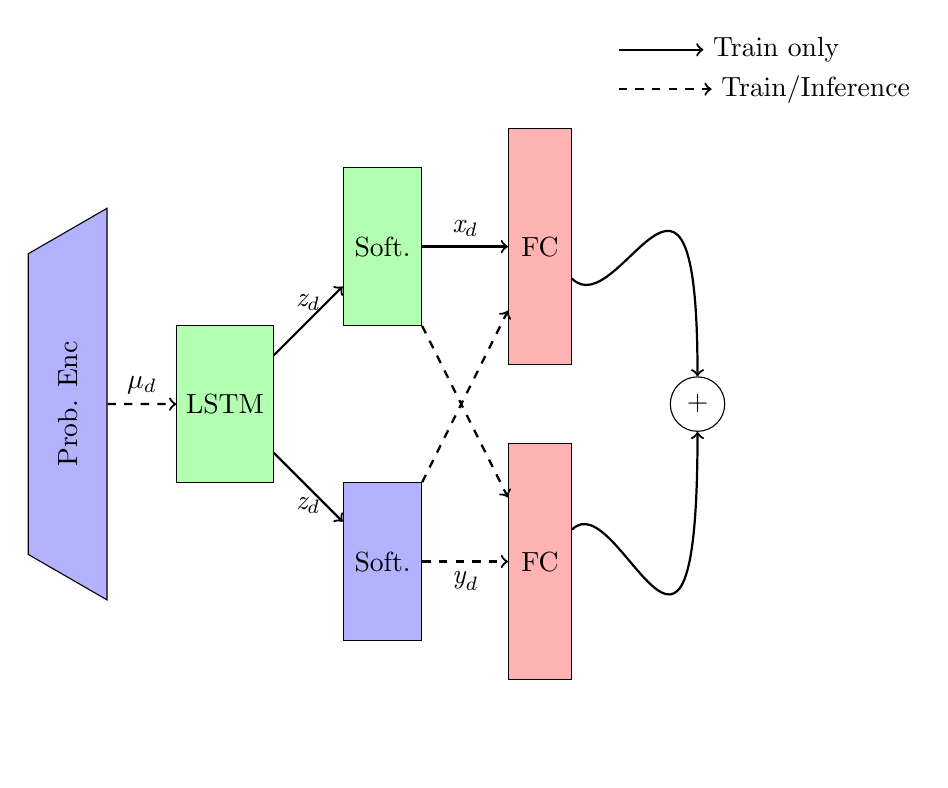
\begin{tikzpicture}[node distance=2cm]

\node at (0,-5) (in1) [io] {Prob. Enc};

\node (pro1) [process1, right of=in1] {LSTM};
\draw[->,dashed,thick](in1) -- node[anchor=south] {$\mu_d$}(pro1);

\node (pro2) [process1, right of=pro1,above of=pro1] {Soft.};
\draw[->,thick](pro1) -- node[anchor=south] {$\textit{z}_d$}(pro2);

\node (pro3) [process2, right of=pro1,below of=pro1] {Soft.};
\draw[->,thick](pro1) -- node[anchor=north] {$\textit{z}_d$}(pro3);

\node (pro4) [process3, right of=pro2] {FC};
\draw[->,thick](pro2) -- node[anchor=south] {$\textit{x}_d$}(pro4);

\node (pro5) [process3, right of=pro3] {FC};
\draw[->,thick,dashed](pro3) -- node[anchor=north] {$\textit{y}_d$}(pro5);

\draw[->,thick,dashed](pro2) -- (pro5);
\draw[->,thick,dashed](pro3) -- (pro4);

\node (circ1) [circ, right of=pro4, below of=pro4] {+};
\draw [->,thick] (pro4) ..controls(7,-4)and(8,-1).. (circ1);
\draw [->,thick] (pro5) ..controls(7,-6)and(8,-9.5).. (circ1);

\node(train1)[textonly] at(9,-0.5) {Train only};
\draw[->,thick] (7,-0.5)-- (train1);

\node(train2)[textonly] at (9.5,-1) {Train/Inference};
\draw[->,thick,dashed] (7,-1)-- (train2);

\end{tikzpicture}
\end{document}
\end{document}
